% 章节支持、单面打印:ctexbook
\documentclass[UTF8,AutoFakeBold,AutoFakeSlant,zihao=-4,oneside,openany]{ctexbook}
\usepackage[a4paper,left=3cm,right=2.6cm,top=3.5cm,bottom=2.9cm]{geometry}
% 目前 29mm 最接近 Word 排版
\usepackage{xeCJK}
\usepackage{titletoc}
\usepackage{fontspec}
\usepackage{setspace}
\usepackage{graphicx}
\usepackage{fancyhdr}
\usepackage{pdfpages}
\usepackage{setspace}
\usepackage{booktabs}
\usepackage{multirow}
\usepackage{caption}
\usepackage{tikz}
\usepackage{etoolbox}
\usepackage[hidelinks]{hyperref}
\usepackage{xcolor}
\usepackage{caption}
\usepackage{array}
\usepackage{amsmath}
\usepackage{amssymb}
\usepackage{pdfpages}

% 设置参考文献编译后端为 biber,引用格式为 GB/T7714-2015 格式
% 参考文献使用宏包见 https://github.com/hushidong/biblatex-gb7714-2015
\usepackage[
  backend=biber,
  style=gb7714-2015,
  gbalign=gb7714-2015,
  gbnamefmt=lowercase,
  gbpub=false,
  doi=false,
  url=false,
  eprint=false,
  isbn=false,
]{biblatex}

% 参考文献引用文件位于 misc/ref.bib
\addbibresource{misc/ref.bib}

% 西文字体默认为 Times New Roman
\setromanfont{Times New Roman}
% 论文题目字体为华文细黑
\setCJKfamilyfont{xihei}{[STXIHEI.TTF]} % 若希望使用本机字体,也可以用 {STXihei} 来调用
\newcommand{\xihei}{\CJKfamily{xihei}}
\newfontfamily\Arial{[ARIALBD.TTF]}
%\newfontfamily\Calibri{Calibri}
% \newfontfamily\Helvetica{Helvetica}

% 在这里填写你的论文中英文题目
\newcommand{\thesisTitle}{北京理工大学本科生毕业设计(论文)题目}
\newcommand{\thesisTitleEN}{The Subject of Undergraduate Graduation Project (Thesis) of Beijing Institute of Technology}

% 在这里填写你的相关信息
\newcommand{\deptName}{School of Mechanical Engineering}
\newcommand{\majorName}{Mechanical Engineering}
\newcommand{\yourName}{Your Name}
\newcommand{\yourStudentID}{112017xxxx}
\newcommand{\mentorName}{Your tutor}
% 如果你的毕设为校外毕设,请将下面这一行语句解除注释(删除第一个百分号字符)并在第二组花括号中填写你的校外毕设导师名字
% \newcommand{\externalMentorName}{左偏树}

% 主题页面格式:BIThesis
\fancypagestyle{BIThesis}{
  % 页眉高度
  \setlength{\headheight}{20pt}
  % 页码高度(不完美,比规定稍微靠下 2mm)
  \setlength{\footskip}{14pt}

  \fancyhf{}
  % 定义页眉、页码
  \fancyhead[C]{\zihao{-4}\songti{Undergraduate Graduation Project (Thesis) of Beijing Institute of Technology}}
  \fancyfoot[C]{\songti\zihao{-5} \thepage}
  % 页眉分割线稍微粗一些
  \renewcommand{\headrulewidth}{0.6pt}
}

% 设置章节格式
% 一级标题:Arial,三号,加粗;间距:段前 0.5 行,段后 1 行;
\ctexset{chapter={
    name = {Chapter\; },
    number = {\arabic{chapter}},
    format = {\Arial \bfseries \centering \zihao{3}},
    aftername = \hspace{9bp},
    pagestyle = BIThesis,
    beforeskip = 8bp,
    afterskip = 32bp,
    fixskip = true,
  }
}

% 二级标题:Arial,四号,加粗;间距:段前 0.5 行,段后 0 行;
\ctexset{section={
    number = {\thechapter.\arabic{section}},
    format = {\Arial \raggedright \bfseries \zihao{4}},
    aftername = \hspace{8bp},
    beforeskip = 20bp plus 1ex minus .2ex,
    afterskip = 18bp plus .2ex,
    fixskip = true,
  }
}

% 三级标题:Arial、小四、加粗;间距:段前 0.5 行,段后 0 行;
\ctexset{subsection={
    number = {\thechapter.\arabic{section}.\arabic{subsection}},
    format = {\Arial \bfseries \raggedright \zihao{-4}},
    aftername = \hspace{7bp},
    beforeskip = 17bp plus 1ex minus .2ex,
    afterskip = 14bp plus .2ex,
    fixskip = true,
  }
}

% 设置目录样式
% 添加 PDF 链接
\addtocontents{toc}{\protect\hypersetup{hidelinks}}

% 解决「目录」二字的格式问题
\renewcommand{\contentsname}{
  \fontsize{16pt}{\baselineskip}
  \Arial{\textbf{Table of Contents}}
  \vspace{-8pt}
}
% 定义目录样式
\titlecontents{chapter}[0pt]{\Calibri\bfseries\zihao{-4}}
{\thecontentslabel\hspace{\ccwd}}{}
{\hspace{.5em}\titlerule*{.}\contentspage}
\titlecontents{section}[1\ccwd]{\Calibri\zihao{-4}}
{\bfseries\thecontentslabel\hspace{\ccwd}}{}
{\hspace{.5em}\titlerule*{.}\contentspage}
\titlecontents{subsection}[2\ccwd]{\Calibri\zihao{-4}}
{\itshape\thecontentslabel\hspace{\ccwd}}{}
{\hspace{.5em}\titlerule*{.}\contentspage}

% 前置页面(原创性声明、中英文摘要、目录等)
\renewcommand{\frontmatter}{
  \pagenumbering{roman}
  \pagestyle{BIThesis}
}

% 正文页面
\renewcommand{\mainmatter}{
  \pagenumbering{arabic}
  \pagestyle{BIThesis}
}

% 设置 caption 与 figure 之间的距离
\setlength{\abovecaptionskip}{11pt}
\setlength{\belowcaptionskip}{9pt}

% 设置图片的 caption 格式
\renewcommand{\thefigure}{\thechapter-\arabic{figure}}
\captionsetup[figure]{font=small,labelsep=space}

% 设置表格的 caption 格式和 caption 与 table 之间的垂直距离
\renewcommand{\thetable}{\thechapter-\arabic{table}}
\captionsetup[table]{font=small,labelsep=space,skip=2pt}

% 调整底层 TeX 排版引擎参数以保证所有段落能够很好地以两端对齐的方式呈现
\tolerance=1
\emergencystretch=\maxdimen
\hyphenpenalty=10000
\hbadness=10000

% 设置数学公式编号格式
\renewcommand{\theequation}{\arabic{chapter}-\arabic{equation}}

\newcommand{\unnumchapter}[1]{
  \chapter*{\vskip 10bp\textmd{#1} \vskip -6bp}
  \addcontentsline{toc}{chapter}{#1}
  \stepcounter{chapter}
}

% Define additional hyperref names
\def\subsectionautorefname{section}
\def\subsubsectionautorefname{section}
\def\subequationsautorefname{Equations}
\newcommand{\subfigureautorefname}{\figureautorefname}

% 文档开始
\begin{document}

% 标题页面:如无特殊需要,本部分无需改动
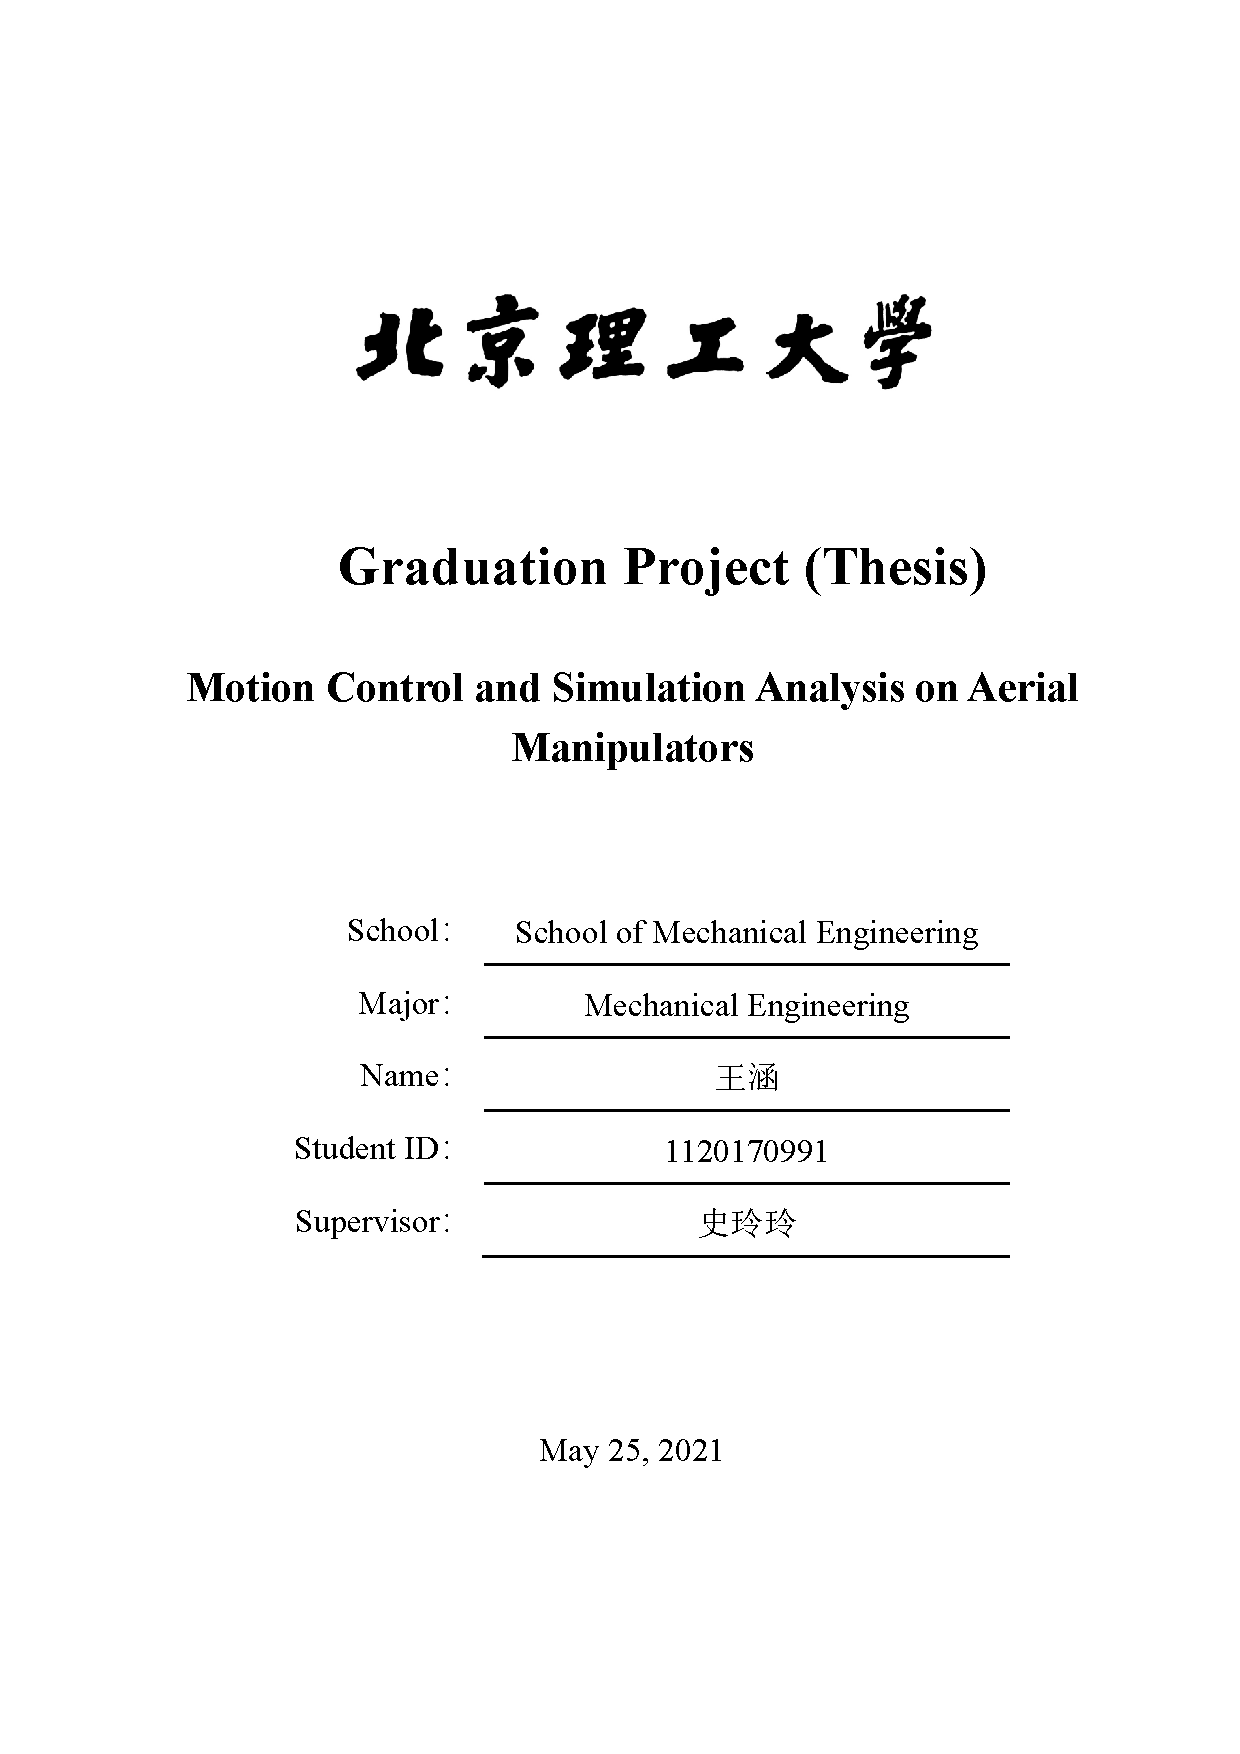
\includepdf[pages=-]{misc/0_cover.pdf}

% 前置页面定义
\frontmatter
% 原创性声明:如无特殊需要,本部分无需改动
% 更改为 PDF 页面插入,如需要添加内容,可考虑先用 Word 制作再覆盖 misc/1_originality.pdf
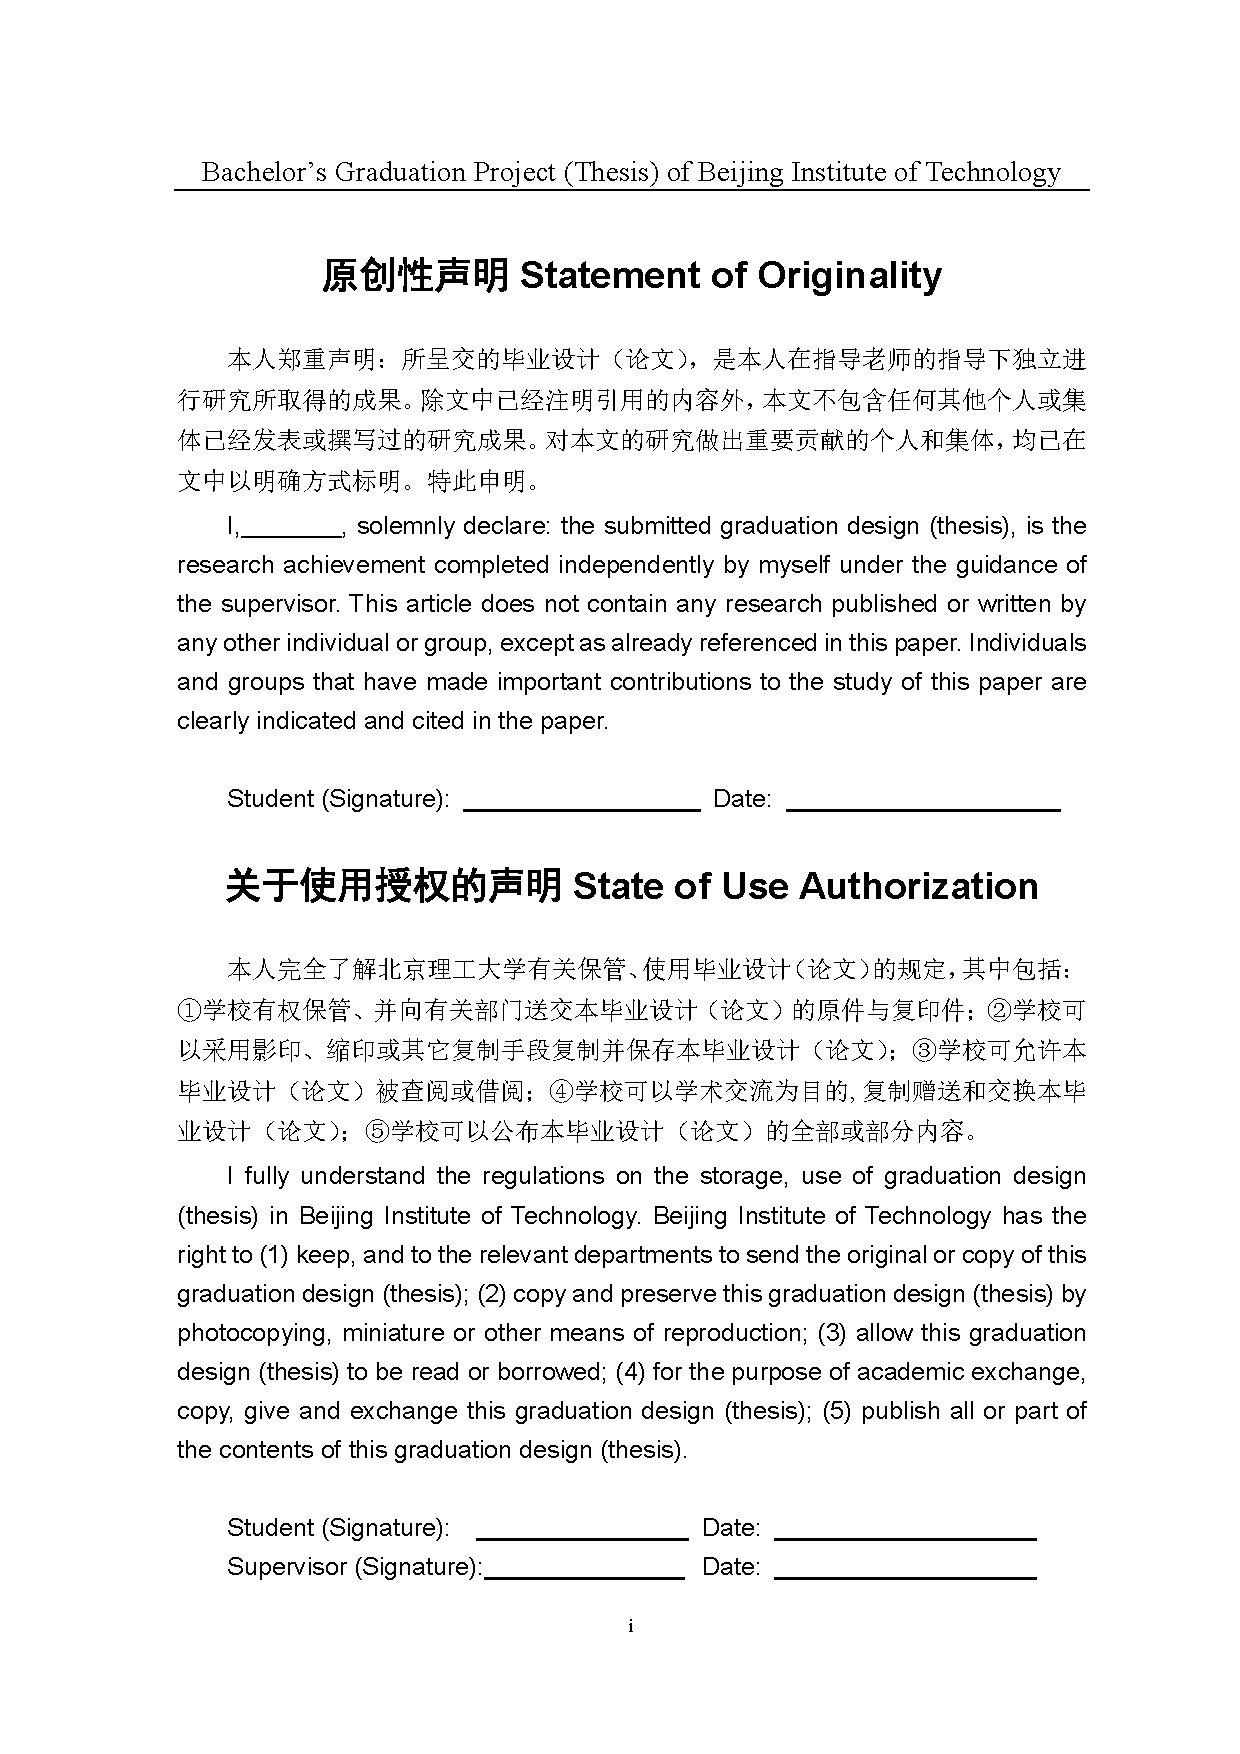
\includepdf{misc/1_originality_en.pdf}
\newpage
%\input{misc/1_originality.tex}
% 摘要:在摘要相应的 TeX 文件处进行摘要部分的撰写
%%
% The BIThesis Template for Bachelor Graduation Thesis
%
% 北京理工大学毕业设计(论文)中英文摘要 —— 使用 XeLaTeX 编译
%
% Copyright 2020 Spencer Woo
%
% This work may be distributed and/or modified under the
% conditions of the LaTeX Project Public License, either version 1.3
% of this license or (at your option) any later version.
% The latest version of this license is in
%   http://www.latex-project.org/lppl.txt
% and version 1.3 or later is part of all distributions of LaTeX
% version 2005/12/01 or later.
%
% This work has the LPPL maintenance status `maintained'.
%
% The Current Maintainer of this work is Spencer Woo.

% 中英文摘要章节
\zihao{-4}
\vspace*{-11mm}

\begin{center}
  \heiti\zihao{3}\textbf{\thesisTitle}
\end{center}

\vspace*{2mm}

{\let\clearpage\relax \chapter*{\zihao{3} \Arial\textbf{Abstract}}}
\addcontentsline{toc}{chapter}{Abstract}
\setcounter{page}{2}

\vspace*{1mm}

\setstretch{1.53}
\setlength{\parskip}{0em}

% % 中文摘要正文从这里开始
In order to study……

% \vspace{4ex}\noindent\textbf{\heiti 关键词:北京理工大学;本科生;毕业设计(论文)}
% \newpage

% % 英文摘要章节
% \vspace*{-2mm}

% \begin{spacing}{0.95}
%   \centering
%   \heiti\zihao{3}\textbf{\thesisTitleEN}
% \end{spacing}

% \vspace*{17mm}

% {\let\clearpage\relax \chapter*{
%   \zihao{-3}\textmd{Abstract}\vskip -3bp}}
% \addcontentsline{toc}{chapter}{Abstract}
% \setcounter{page}{2}

% \setstretch{1.53}
% \setlength{\parskip}{0em}

% % 英文摘要正文从这里开始
% In order to study……

% \textcolor{blue}{Abstract 正文设置成每段落首行缩进 2 字符,字体:Times New Roman,字号:小四,行距:固定值 22 磅,间距:段前、段后均为 0 行。阅后删除此段。}

\vspace{3ex}\noindent\textbf{Key Words}: BIT; Undergraduate; Graduation Project (Thesis)
\newpage

% 目录:如无特殊需要,本部分无需改动
%%
% The BIThesis Template for Bachelor Graduation Thesis
%
% 北京理工大学毕业设计(论文)目录 —— 使用 XeLaTeX 编译
%
% Copyright 2020 Spencer Woo
%
% This work may be distributed and/or modified under the
% conditions of the LaTeX Project Public License, either version 1.3
% of this license or (at your option) any later version.
% The latest version of this license is in
%   http://www.latex-project.org/lppl.txt
% and version 1.3 or later is part of all distributions of LaTeX
% version 2005/12/01 or later.
%
% This work has the LPPL maintenance status `maintained'.
%
% The Current Maintainer of this work is Spencer Woo.
%
% 如无特殊需要,本页面无需更改

% 目录开始

% 调整目录行间距
\renewcommand{\baselinestretch}{1.53}
% 目录
\tableofcontents
\newpage


% 正文开始
\mainmatter
% 正文 22 磅的行距
\setlength{\parskip}{0em}
\renewcommand{\baselinestretch}{1.53}
% 修复脚注出现跨页的问题
\interfootnotelinepenalty=10000

% % 第一章
% \input{chapters/1_chapter1.tex}
% % 在这里添加第二章、第三章……TeX 文件的引用
% % \input{chapters/2_chapter2.tex}
% % \input{chapters/3_chapter3.tex}

% % 结论:在结论相应的 TeX 文件处进行结论部分的撰写
\chapter*{Conclusion}
\addcontentsline{toc}{chapter}{Conclusion}


% % 参考文献:如无特殊需要,参考文献相应的 TeX 文件无需改动,添加参考文献请使用 BibTeX 的格式
% %   添加至 misc/ref.bib 中,并在正文的相应位置使用 \cite{xxx} 的格式引用参考文献
% %%
% The BIThesis Template for Bachelor Graduation Thesis
%
% 北京理工大学毕业设计(论文)参考文献 —— 使用 XeLaTeX 编译
%
% Copyright 2020 Spencer Woo
%
% This work may be distributed and/or modified under the
% conditions of the LaTeX Project Public License, either version 1.3
% of this license or (at your option) any later version.
% The latest version of this license is in
%   http://www.latex-project.org/lppl.txt
% and version 1.3 or later is part of all distributions of LaTeX
% version 2005/12/01 or later.
%
% This work has the LPPL maintenance status `maintained'.
%
% The Current Maintainer of this work is Spencer Woo.
%
% Compile with: xelatex -> biber -> xelatex -> xelatex
%
% 如无特殊需要,本页面无需更改

% 参考文献开始
\unnumchapter{\bfseries References}
\renewcommand{\thechapter}{References}

% 设置参考文献字号为 5 号
\renewcommand*{\bibfont}{\zihao{5}}
% 设置参考文献各个项目之间的垂直距离为 0
\setlength{\bibitemsep}{0ex}
\setlength{\bibnamesep}{0ex}
\setlength{\bibinitsep}{0ex}
% 设置单倍行距
\renewcommand{\baselinestretch}{1.2}
% 设置参考文献顺序标签 `[1]` 与文献内容 `作者. 文献标题...` 的间距
\setlength{\biblabelsep}{0.5mm}
% 设置参考文献后文缩进为 0(与 Word 模板保持一致)
\renewcommand{\itemcmd}{
  \addvspace{\bibitemsep} % 恢复 \bibitemsep 的作用
  \mkgbnumlabel{\printfield{labelnumber}}
  \hspace{\biblabelsep}}

% 删除默认的「参考文献 / Reference」标题,使用上面定义的 section 标题
\printbibliography[heading=none]

% % 附录:在附录相应的 TeX 文件处进行附录部分的撰写
% %%
% The BIThesis Template for Bachelor Graduation Thesis
%
% 北京理工大学毕业设计(论文)附录 —— 使用 XeLaTeX 编译
%
% Copyright 2020 Spencer Woo
%
% This work may be distributed and/or modified under the
% conditions of the LaTeX Project Public License, either version 1.3
% of this license or (at your option) any later version.
% The latest version of this license is in
%   http://www.latex-project.org/lppl.txt
% and version 1.3 or later is part of all distributions of LaTeX
% version 2005/12/01 or later.
%
% This work has the LPPL maintenance status `maintained'.
%
% The Current Maintainer of this work is Spencer Woo.
%
% Compile with: xelatex -> biber -> xelatex -> xelatex

\unnumchapter{\bfseries Appendix}
\renewcommand{\thechapter}{Appendix}

% 设置附录编号格式
\ctexset{
  section/number = Appendix \Alph{section}
}

Contents here

% 这里示范一下添加多个附录的方法:

\section{\LaTeX Env}
\LaTeX Env。

\section{BIThesis 使用说明}
BIThesis 使用说明。


% % 致谢:在致谢相应的 TeX 文件处进行致谢部分的撰写
% %%
% The BIThesis Template for Bachelor Graduation Thesis
%
% 北京理工大学毕业设计(论文)致谢 —— 使用 XeLaTeX 编译
%
% Copyright 2020 Spencer Woo
%
% This work may be distributed and/or modified under the
% conditions of the LaTeX Project Public License, either version 1.3
% of this license or (at your option) any later version.
% The latest version of this license is in
%   http://www.latex-project.org/lppl.txt
% and version 1.3 or later is part of all distributions of LaTeX
% version 2005/12/01 or later.
%
% This work has the LPPL maintenance status `maintained'.
%
% The Current Maintainer of this work is Spencer Woo.
%
% Compile with: xelatex -> biber -> xelatex -> xelatex

\unnumchapter{\bfseries Acknowledgements}
\renewcommand{\thechapter}{Acknowledgements}

\ctexset{
  section/number = \arabic{section}
}

% 致谢部分尽量不使用 \subsection 二级标题,只使用 \section 一级标题

值此论文完成之际,首先向我的导师……




\chapter{This is a chapter}
\section{This is a section}
\subsection{This is a subsection}
\subsubsection{This is a subsubsection}
\begin{equation}\label{Eq:sample_eq}
    e^{\pi i} + 1 =0
\end{equation}
\autoref{Eq:sample_eq} is a sample equation.
%%
% The BIThesis Template for Bachelor Graduation Thesis
%
% 北京理工大学毕业设计(论文)参考文献 —— 使用 XeLaTeX 编译
%
% Copyright 2020 Spencer Woo
%
% This work may be distributed and/or modified under the
% conditions of the LaTeX Project Public License, either version 1.3
% of this license or (at your option) any later version.
% The latest version of this license is in
%   http://www.latex-project.org/lppl.txt
% and version 1.3 or later is part of all distributions of LaTeX
% version 2005/12/01 or later.
%
% This work has the LPPL maintenance status `maintained'.
%
% The Current Maintainer of this work is Spencer Woo.
%
% Compile with: xelatex -> biber -> xelatex -> xelatex
%
% 如无特殊需要,本页面无需更改

% 参考文献开始
\unnumchapter{\bfseries References}
\renewcommand{\thechapter}{References}

% 设置参考文献字号为 5 号
\renewcommand*{\bibfont}{\zihao{5}}
% 设置参考文献各个项目之间的垂直距离为 0
\setlength{\bibitemsep}{0ex}
\setlength{\bibnamesep}{0ex}
\setlength{\bibinitsep}{0ex}
% 设置单倍行距
\renewcommand{\baselinestretch}{1.2}
% 设置参考文献顺序标签 `[1]` 与文献内容 `作者. 文献标题...` 的间距
\setlength{\biblabelsep}{0.5mm}
% 设置参考文献后文缩进为 0(与 Word 模板保持一致)
\renewcommand{\itemcmd}{
  \addvspace{\bibitemsep} % 恢复 \bibitemsep 的作用
  \mkgbnumlabel{\printfield{labelnumber}}
  \hspace{\biblabelsep}}

% 删除默认的「参考文献 / Reference」标题,使用上面定义的 section 标题
\printbibliography[heading=none]

%%
% The BIThesis Template for Bachelor Graduation Thesis
%
% 北京理工大学毕业设计(论文)附录 —— 使用 XeLaTeX 编译
%
% Copyright 2020 Spencer Woo
%
% This work may be distributed and/or modified under the
% conditions of the LaTeX Project Public License, either version 1.3
% of this license or (at your option) any later version.
% The latest version of this license is in
%   http://www.latex-project.org/lppl.txt
% and version 1.3 or later is part of all distributions of LaTeX
% version 2005/12/01 or later.
%
% This work has the LPPL maintenance status `maintained'.
%
% The Current Maintainer of this work is Spencer Woo.
%
% Compile with: xelatex -> biber -> xelatex -> xelatex

\unnumchapter{\bfseries Appendix}
\renewcommand{\thechapter}{Appendix}

% 设置附录编号格式
\ctexset{
  section/number = Appendix \Alph{section}
}

Contents here

% 这里示范一下添加多个附录的方法:

\section{\LaTeX Env}
\LaTeX Env。

\section{BIThesis 使用说明}
BIThesis 使用说明。


%%
% The BIThesis Template for Bachelor Graduation Thesis
%
% 北京理工大学毕业设计(论文)致谢 —— 使用 XeLaTeX 编译
%
% Copyright 2020 Spencer Woo
%
% This work may be distributed and/or modified under the
% conditions of the LaTeX Project Public License, either version 1.3
% of this license or (at your option) any later version.
% The latest version of this license is in
%   http://www.latex-project.org/lppl.txt
% and version 1.3 or later is part of all distributions of LaTeX
% version 2005/12/01 or later.
%
% This work has the LPPL maintenance status `maintained'.
%
% The Current Maintainer of this work is Spencer Woo.
%
% Compile with: xelatex -> biber -> xelatex -> xelatex

\unnumchapter{\bfseries Acknowledgements}
\renewcommand{\thechapter}{Acknowledgements}

\ctexset{
  section/number = \arabic{section}
}

% 致谢部分尽量不使用 \subsection 二级标题,只使用 \section 一级标题

值此论文完成之际,首先向我的导师……




\end{document}
